\chapter{Data and Research Design}
\label{data}

In our simulation we will compare welfare effects of default lifecycles and individualized lifecycles defined below. The magnitutes and sources of parameters are given in the next section. Default lifecycles are taken from the ones mentioned in our Literature Review chapter and from the real investment strategies of the largest Turkish pension fund provider Anadolu Hayat Emeklilik. Individualized lifecycles will be calculated using Munk's optimal portfolio formula from previous chapter taking idiosyncracies into consideration.

\section{Data}

To measure the stock series we used BIST 30 index which measures the aggregate performance of 30 best companies in Turkey. The monthly data is taken from Borsa Istanbul. We can see from Figure 4.1 the general upward trend with collapse during 2008 crisis.

\begin{figure}
	\centering
    \begin{minipage}{0.45\textwidth}
		\centering
		\includegraphics[scale=0.4]{figs/bist.pdf}
		\caption{BIST30 Turkish stock market performance index}
	\end{minipage}
	\hfill
    \begin{minipage}{0.45\textwidth}
		\centering
		\includegraphics[scale=0.4]{figs/reidin.pdf}
		\caption{Reidin Turkish house price index}
	\end{minipage}
\end{figure}

\paragraph{}We used Reidin AEINDEXF index to obtain data on house prices in Istanbul. The historical dynamics of this index are illustrated in Figure 4.2.

\paragraph{}We used TUIK's Household Budget Survey Data and regression results of Aktug, Kuzubas, Torul (2017). We have 55 thousand panel data points for 170 households for 2001 to 2014 years. We can observe the hump-shaped lifetime income distribution in Figure 4.3. This corresponds well to an established literature in this field.

\begin{figure}[h]
	\centering
	\includegraphics[scale=0.6]{figs/wage2median.pdf}
	\caption{Median Turkish salaries by age}
\end{figure}

\subsection{Default parameters}
In our simulation we start with a 28 years old individual who invests in her retirement for 30 years until she reaches retirement at 57. In line with Torul et al. (2018) we set the coefficient of relative risk aversion for Turkey at $1.5$, and the subjective discount rate at $0.89$.

\paragraph{}Stock returns for Turkey were estimated from historical data to be equal to $23.2\%$ annually, with variance $36\%$. Risk-free rate forecasts are obtained from OECD Data Bank (2018) and are equal to $10.8\%$ per annum.

\paragraph{}Housing capital appreciation averaged at $8.3\%$ with $9.5\%$ variance. Aggregate wage growth series showed $5.5\%$ standard deviation.

\paragraph{}The correlations between house and stock prices, and house prices and wages gave $0.24$ and $0.37$ respectively.

\paragraph{}The data on survival probability for all ages has been taken from Turkish Statistical Institute's (TUIK) database and illustrated in Figure 4.4. All of these findings have been summarized in Table 4.1. 

\begin{figure}[h]
	\centering
	\includegraphics[scale=0.6]{figs/survival.pdf}
	\caption{Survival probabilities by age}
\end{figure}

\begin{table}
	\centering
	\caption{Benchmark Parameters}
	\begin{tabular}[c]{lll}
		\hline
		Parameter&Description&Value\\
		\hline
		$Y$&Beginning age&$28$\\
		$R$&Retirement age&$57$\\
		$T$&Lifespan (years)&$100$\\
		$\gamma$&Risk aversion&$1.5$\\
		$\beta$&Discount rate&$0.89$\\
		$r_f$&Risk-free rate&$0.108$\\
		$\pi$&Average inflation rate&$0.084$\\
		\hline
		$\mu_s$&Expected stock returns&$0.232$\\
		$\mu_h$&Expected housing returns&$0.083$\\
		$\sigma_s$&Stock returns volatility&$0.36$\\
		$\sigma_h$&Housing returns volatility&$0.095$\\
		$\sigma_w$&Wage growth volatility&$0.056$\\
		$\rho_{hs}$&Housing-stock correlation&$0.24$\\
		$\rho_{hw}$&Housing-wage correlation&$0.37$\\
		\hline
		$p_{28}$&Survival probability at age 28&$0.977$\\
		$p_{57}$&Survival probability at age 57&$0.924$\\
		$p_{100}$&Survival probability at age 100&$0$\\	
		\hline
	\end{tabular}
\end{table}


\subsection{Heterogeneity parameters}
In the same manner as Olear(2014) we will use wage growth rate, stock-income correlation and idiosyncratic labor income risk to model heterogeneities in education and sector. Let's now consider the heterogeneities one at a time:

\subsubsection{Heterogeneity in education}
In line with Olear's (2016) approach we model the heterogeneity in education using the differences in wage growth rates. Indeed, we expect the salaries for higher education level to grow faster than for the lower education level. Some of this expectation comes from the fact that people with lower education are restricted in their career ladders and cannot rise very high in a workplace. Another intuition is that while college dropouts start working immediately, college graduates and graduate students continue to study and thus report zero income. When they graduate, their salary immediately rises from zero to the average salary, and this constitutes a steeper wage growth curve at the beginning of their lives. Figure 4.5 shows the wage series for different levels of education. Note that the curves for the lowest education levels are practically flat and the those for the highest education levels have varying non-zero slopes. 

\begin{figure}[h]
	\centering
	\includegraphics[scale=0.6]{figs/wage2educ.pdf}
	\caption{Lifetime wage dynamics by education level}
\end{figure}

Performing kinked regressions of log wages on ages yielded best linear fits for three different education levels of our choice: postgraduate, high school, and no schooling. The corresponding labor income growth rates can be characterized as steep, moderate, and flat respectively. We considered wage data until 60 years, as Turkish retirement age is at 57, and have added empirically best kinks at ages 35 and 45. The results are summarized in Table 4.2 and illustrated in Figure 4.6. In this figure red lines represent the actual wages dynamics for postgraduate, high school, and no schooling, and blue lines are plots of the percentage changes proposed in Table 4.2, where the starting points all correspond to the actual starting points from the data. Figure 4.7 illustrates the same parameterized curves without actual wage curves. 

\begin{table}
	\centering
	\caption{Estimated Benchmark Wage Growth Rates $\mu_w$}
	\begin{tabular}[c]{l|ccc}
		Age&Flat&Moderate&Steep\\
		\hline
		0-35&0\%&3.5\%&6.5\%\\
		36-45&0\%&3\%&2\%\\
		46-60&0\%&0\%&0\%\\
	\end{tabular}
\end{table}


\begin{figure}[h]
	\centering
    \begin{minipage}{0.45\textwidth}
		\centering
		\includegraphics[scale=0.4]{figs/heterwage.pdf}
		\caption{Actual and parameterized benchmark wage dynamics by age}
	\end{minipage}
	\hfill
    \begin{minipage}{0.45\textwidth}
		\centering
		\includegraphics[scale=0.4]{figs/heterwageless.pdf}
		\caption{Parameterized wage dynamics by age}
	\end{minipage}

\end{figure}


\subsubsection{Heterogeneity in sectors of work}

As we explained in Chapter 3, we model our labor income series as functions of age, gender, education, sector of work etc. We already showed in previous section how we incorporated the heterogeneity in education. We also stated at the beginning of this chapter that we consider only male individuals as heads of households; age is implicit in our analysis. In this section we will model the differences in sectors of work. Again, similar to Olear's (2016) approach we model these differences using correlations of wage growth rates with stock market returns. Indeed, it is expected that sectoral wages would be proportional to the stock returns only to the extent of their exposure to stock markets. In that sense, the stock-wage correlations are expected to be zero for public sector, where wages are fixed regardless the markets, and high in financial institutions. When we juxtaposed wages by sector and stock prices we obtained very high correlations, which was expected due to the economic growth over the years represented in Figure 4.8. Therefore we divided the wages by price levels to obtain the real wages, and, as expected, we obtained more realistic correlations. The financial sector's correlations were as high as $0.44$  and public sector, social service and education's were as low as $0.08$. Thus, our expectations that different sectors have different wage-stock correlation $\rho_{sw}$ were confirmed and we decided on three measures of $\rho_{sw}$ as our simulation benchmarks: $0$, $0.2$ and $0.4$ as stated in Table 4.3.

\begin{figure}[h]
	\centering
	\includegraphics[scale=0.6]{figs/wage2sec.pdf}
	\caption{Historical wage dynamics by sector}
\end{figure}

\begin{table}
	\centering
	\caption{Benchmark Wage to Stock Correlations}
	\begin{tabular}[c]{c|ccc}
		&Low&Moderate&High\\
		\hline
		$\rho_{sw}$&0&0.2&0.4
	\end{tabular}
\end{table}


\subsubsection{Individual heterogeneity}

We model individual heterogeneity using idiosyncratic labor income shocks $\sigma_{\epsilon}$. We consider three different values $0.03$,$0.05$ and $0.07$. Total variance is calculated, as stated in previous chapter, as a sum of squares of aggregate and idiosyncratic shocks $\sigma^2_W = \sigma^2_w + \sigma^2_{\epsilon}$. This heterogeneity is summarized in Table 4.4. 


\begin{table}
	\centering
	\caption{Benchmark Wage Volatilities and Their Sum of Squares}
	\begin{tabular}[c]{l|ccc}
		&Low&Moderate&High\\
		\hline
		$\sigma_w$&$0.056$&$0.056$&$0.056$\\
		$\sigma_{\epsilon}$&$0.03$&$0.05$&$0.07$\\
		\hline
		$\sigma^2_{W}$&$0.004$&$0.0056$&$0.008$
	\end{tabular}
\end{table}


\subsubsection{Housing wealth heterogeneity}

Apart from the above three heterogeneities, all related to labor income process, we also consider differences in housing wealth to match Munk's (2016) approach completely. We have SOMETHING ABOUT H ZERO ET CETERA...



\section{Capital series}

\subsection{Human capital}
Human capital at all ages has been calculated as a discounted sum of all future wages until retirement with the discount factor $r_f$. To construct the individualized capital we used steep, moderate and flat wage series mentioned in the previous section. It can be seen in Figure 4.9 that human capital is declining for flat wages and hump-shaped for moderate and steep wages. 

\begin{figure}[h]
	\centering
    \begin{minipage}{0.45\textwidth}
		\centering
		\includegraphics[scale=0.4]{figs/humancapital.pdf}
		\caption{Human capital by age}
	\end{minipage}
	\hfill
    \begin{minipage}{0.45\textwidth}
		\centering
		\includegraphics[scale=0.4]{figs/fincapital.pdf}
		\caption{Financial capital by age}
	\end{minipage}
\end{figure}

\subsection{Financial capital}

Financial capital evolves according to dynamic investment illustrated in Figure 4.11. Every period $t$ a certain percentage $c$ (equal to $3\%$ in Turkey) of that period's wage $w_t$ is invested in a retirement portfolio. At the same time, the previously invested amount accrues interest. We started with 28 years old individual who invests for 30 years until retirement, as has been mentioned previously numerous times.

\begin{figure}[h]
	\centering
	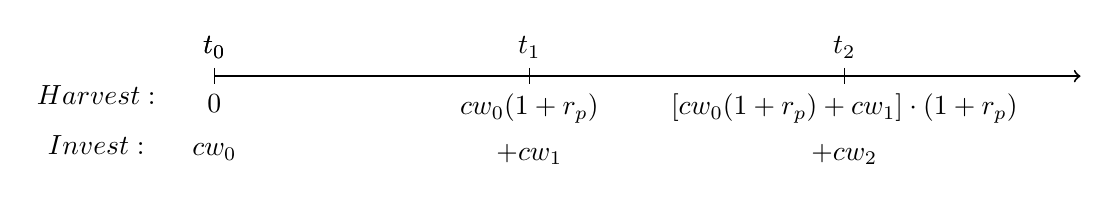
\begin{tikzpicture}
		\draw [->, line width=0.25mm] (0,0) -- (11,0);
		\foreach \x in {0,4,8}
			\draw (\x cm,3pt) -- (\x cm, -3pt);
		\draw (0,0) node[below=21pt] {$ cw_0 $} node[above=3pt] {$ t_0 $};
    	\draw (4,0) node[below=21pt] {$ +cw_1 $} node[above=3pt] {$ t_1 $};
    	\draw (8,0) node[below=21pt] {$ +cw_2 $} node[above=3pt] {$ t_2 $};
		\draw (0,0) node[below=3pt] {$ 0 $} node[above=3pt] {$ t_0 $};
    	\draw (4,0) node[below=3pt] {$ cw_0(1+r_p) $};
    	\draw (8,0) node[below=3pt] {$ \left[cw_0(1+r_p) + cw_1 \right] \cdot (1+r_p) $};
	    \draw (-1.5,0) node[below=18pt] {$ Invest: $};
    	\draw (-1.5,0) node[below=0pt] {$ Harvest: $};
	\end{tikzpicture}
	\caption{Law of motion of financial capital}
\end{figure}

\paragraph{}Note that the shape of the financial capital depends on $r_p$ - the rate of return on portfolio, which itself depends on the risky-to-riskless asset ratio. Different such ratios are listed and analyzed in detail in the next section. Figure 4.10 demonstrates the evolution of financial capital for two investment options, provided by Anadolu Hayat Emeklilik - $30\%$ in stocks and $70\%$ in bonds, and by solving Markowitz's formula - $63\%$ in stocks and $37\%$ in bonds.

\paragraph{}It is important to notice here that since human capital is declining by age and financial capital is increasing, the ratio $\frac{L_t}{F_t}$ is declining in $t$. Recalling Merton's formula for $\alpha_t$ from Chapter 2, $\frac{\mu - R_f}{\gamma \sigma^2}(1+\frac{L_t}{F_t})$, it should be now clear how the above fraction creates a lifecycle effect - different ratios for different ages. 

\subsection{Housing capital}




\section{Investment strategies}
\subsection{Default lifecyccles}
As was discussed in the previous chapter, our individual decides between investing in risky (stocks) or risk-free (bonds) assets. The default allocations for share of risky asset are given by:

\begin{itemize}
	\item $100-t$, for all $t$
	\item $\begin{cases} 100\%, & t<40\\(200-2.5t)\%, & t\in[40,57]\end{cases}$
	\item $63\%$, for all $t$
	\item $30\%$, for all $t$
\end{itemize}

where the latter two are Markowitz's solution and Anadolu Hayat's moderate investment option respectively. Since we are only interested in age span between 28 and 57, Figure 4.9 shows the risky asset share $\pi_t$ only for that interval. 

\begin{figure}[h]
	\centering
	\includegraphics[scale=0.6]{figs/defaults.pdf}
	\caption{Default portfolio allocations of stock investments}
\end{figure}


\subsection{Individualized lifecycles}

To derive individualized lifecycle strategies, we used Merton's (1971) and Munk's (2016) optimal portfolio allocation formulas mentioned in chapters 2 and 3. Since these formulas depended on intratemporal amounts of capital, we have constructed three human capital series corresponding to flat, moderate and steep wage growth curves mentioned in the previous section. Figure 4.10 illustrates the risky asset shares given by Merton and Munk. 

\begin{figure}[h]
	\centering
	\includegraphics[scale=0.6]{figs/individuals.pdf}
	\caption{Individual portfolio allocations of stock investments}
\end{figure}
